\documentclass[conference]{IEEEtran}
\ifCLASSINFOpdf

\else

\fi
\usepackage{graphicx}
\hyphenation{op-tical net-works semi-conduc-tor}


\begin{document}
%
% paper title
% can use linebreaks \\ within to get better formatting as desired
% Do not put math or special symbols in the title.
\title{Intelligent Cylindrical Capacitive Level Sensor }


% author names and affiliations
% use a multiple column layout for up to three different
% affiliations
\author{\IEEEauthorblockN{Srikanth Malla}
\IEEEauthorblockA{B.Tech, VIT University,\\ Vellore, 632014,\\ India\\
Email: malla.srikanth2012@vit.ac.in}
\and
\IEEEauthorblockN{Venkata Lakshmi Narayana.K}
\IEEEauthorblockA{ Program Chair, SELECT,\\ VIT University,\\ Vellore, 632014,\\ India\\
Email: kvlnarayana@vit.ac.in}}

% make the title area
\maketitle

% As a general rule, do not put math, special symbols or citations
% in the abstract
\begin{abstract}
The  capacitive  level  sensors  are  most  commonly  used  sensors  for  the  measurement  of  liquid level in  the  industries. It  is  because  of  their  high  sensitivity,  less  power  dissipation  and ruggedness in design. However, in a capacitance sensor, the problem of high nonlinear response characteristics as well as dependence on the permittivity of liquid have imposed some restriction on the optimal use of such sensors. This paper compares different soft-computing algorithms and their performances. 

\end{abstract}

% no keywords




% For peer review papers, you can put extra information on the cover
% page as needed:
% \ifCLASSOPTIONpeerreview
% \begin{center} \bfseries EDICS Category: 3-BBND \end{center}
% \fi
%
% For peerreview papers, this IEEEtran command inserts a page break and
% creates the second title. It will be ignored for other modes.
\IEEEpeerreviewmaketitle



\section{Introduction}
% no \IEEEPARstart
There can be many direct and indirect methods for increasing the linearity of sensor response. ANN applies one such method. The advantages of using ANN for increasing the linearity range are ease of programming and software portability. It uses the synaptic weights for the training to minimize the error between the desired output and the actual output. After training the hardwired version of neural network (with fixed synaptic weights) can be cascaded with the sensor in order to cancel the sensor’s nonlinear characteristics. [1]\\
Jagdish Chandra Patra et al. propose Neural networks based scheme, when there is a change in ambient temperature, the ANN automatically compensates for this change based on the learning which it undergoes and on the information stored in its weights. The effect of change in environmental conditions on the capacitive sensors and subsequently upon the output is nonlinear in nature. Especially, change in ambient temperature causes response characteristics of the sensor to become highly nonlinear, and complex signal processing may be required to obtain correct readout. The purpose of direct modeling is to obtain an ANN model of the sensor in such a way that the outputs of the sensor and the ANN match closely. ANN model has been found to be capable of accurately estimating at any ambient temperature from $20^o$C to $70^o$C. This fact is the novel characteristic of the proposed ANN model. [2]\\
Artificial neural networks have emerged as a powerful learning technique to perform complex tasks nonlinear dynamic environments. An intelligent pressure sensor based on artificial neural networks to realize auto-calibration and nonlinear compensation of a CPS has been proposed with quite satisfactory performance. This technique can also be applied for other parameters such level etc. There are also some drawbacks of neural networks, such as neural networks can’t tell the redundant information from a huge amount of data, which will easily lead to some problems such as long training time and much computation. [3]\\
As explained in the paper [4], the nonlinear operation of a Multi layer perceptron (MLP) neural network compensates the nonlinear characteristics of a sensor. Sensor linearization can be considered a function estimation (modeling) task, where the non-linear sensor output can be used as input data and the desired linearized response as target data. 
The capability of a trained network can be measured to some extent by the errors on the training, validation and test sets. This can be done by applying unseen input to network and trace the output and compare with the sensor output. It has been proved successful in representing any measurable function within any desired degree of accuracy, with the correct values of pressures and sufficient number of hidden neurons. [5]

\section{Hardware Description}
\begin{table}[htdp]
\begin{center}
  \begin{tabular}{ | l | c |}
    \hline
    Power supply   & 24V DC (2wire system) \\ \hline
    Probe size     & 1/4 inch dia probe with high\\ 
                   & temperature standoff \\ \hline
    Type of probe  & Dual Probe \\ \hline
    output         & 4-20mA DC \\ \hline
    Capacitance range  & 0pF(min) to 5nF(max) \\ \hline
  \end{tabular}
\end{center}
\caption{hardware description\label{tab:a}}
\end{table}
Switzer manufacturer’s capacitive level transmitter is used for the experimentation, whose specifications are shown in the Table 1.

\section{Methodology}
\subsection{Back Propagation Neural Network}
The back propagation NN is trained using gradient descent algorithm, which updates the weights to minimize the error, in each epoch as shown in equation 1 and the error is shown in equation 2\\
\begin{equation} \label{eq:1}
W_{n+1} = W_n-\eta \frac{dE}{dW_n}
\end{equation}

\begin{equation} \label{eq:2}
E = 0.5 ||target-output||^2
\end{equation}\\
\\
Where,\\
$\eta$ is the learning rate $0<\eta<1$, \\
$W_i$ is value of weights at $i_{th}$ epoch

\begin{figure}[h]
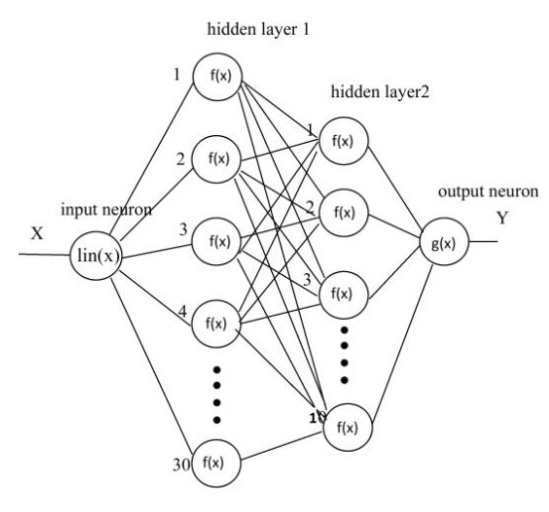
\includegraphics[width=8cm]{net.png}
\centering
\caption{Single Hidden Layer Neural Network Structure\label{Fig:1}}
\end{figure}
It is a generalization of the delta rule to multi-layered feedforward networks, made possible by using the chain rule to iteratively compute gradients for each layer. The 
architecture of the neural network used is shown in Figure 1.

\subsection{RBF Neural Network}
Here we use Gaussian function as the radial basis function, shown in equation 3. It can also be interpreted as a rather simple single-layer type of artificial neural network called a radial basis function network, with the radial basis functions taking on the role of the activation functions of the network. The means of the hidden layer are computed using K means clustering using k as number of hidden neurons.

\begin{equation} \label{eq:3}
\Phi(x) =   {e} ^ {\frac{- {||x-W||} ^ {2}}{{\sigma} ^ {2}}}
\end{equation}\\
\\Where,\\
$\sigma^2$ is variance,\\
x is input, $\Phi(x)$ is output of neuron\\
W is the mean of the sigmoid function or weight of neuron\\

\subsection{Extreme learning Machine}
ELM is one step training algorithm, it uses least squares method to estimate the best fit for the weights of the neural network. \\
Here output layer weights are computed, where the hidden layer weights are assigned to the random value. The hidden layer output matrix is assigned as H as shown in equation 4. Output weights $W_{out}$ are calculated as shown in equation 5.
\begin{equation} \label{eq:4}
H=XW_{hidden}^T+b_{hidden}
\end{equation}
\begin{equation} \label{eq:5}
W_{out}^T=H^+(y-b_{out})
\end{equation}
\\Where,\\
y is the target data,\\
$H^+$ is the pseudo inverse of H,\\
$b_{hidden}$ is the hidden layer bias vector,\\
$b_{out}$ is output layer bias vector.\\
\subsection{Signal conditioning}
The frequency output of the 555 timer varies with the input capacitance in accordance with $(R_1+2R_2)$ as shown in equation 6.\\
\begin{equation}\label{eq:6}
f=\frac{1}{ln (2)C(R_1+2R_2)}
\end{equation}
Where, \\
f is the frequency output and R1=1MΩ, R2=100KΩ\\

The circuit diagram of capacitance to frequency is shown in Figure 2.
\begin{figure}[h]
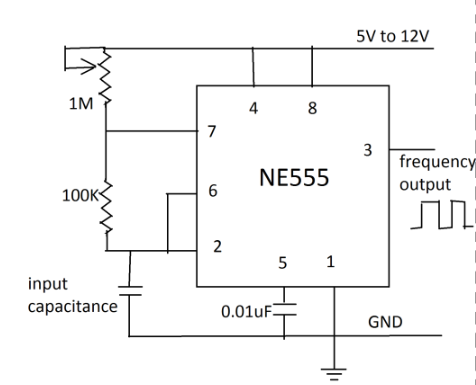
\includegraphics[width=8cm]{ctof.png}
\centering
\caption{capacitance to frequency circuit diagram}\label{Fig2}
\end{figure}
\\The high time and the low time in each pulse is given by equation 7 and equation 8 respectively.\\
\begin{equation} \label{eq:7}
t_{high}= ln(2)C(R_1+R_2)                    
\end{equation}
\begin{equation} \label{eq:8}
t_{low}= ln(2)CR_2                          
\end{equation}
The frequency to voltage converter uses LM331 IC as shown in Figure 3. $R_3$ resistance value depends on the supply voltage as shown in equation 9. The output voltage is obtained as shown in equation 10.\\

\begin{equation} \label{eq:9}
 R3= \frac{V_s-2}{2}1000\ \ \Omega           
 \end{equation}               
\begin{equation} \label{eq:10}
V_{out} = 2.09\frac{R_4}{R_5+R_6}R_1C_1VF_{in}  
\end{equation}            
\begin{figure}[h]
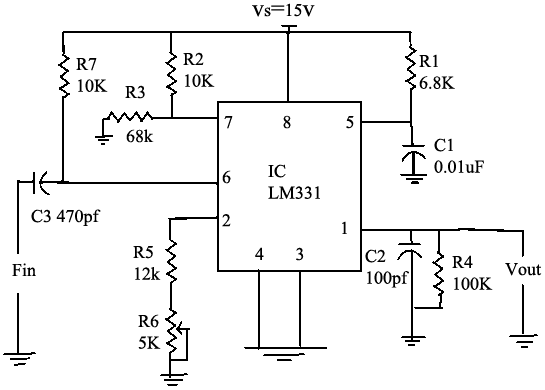
\includegraphics[width=8cm]{ftov.png}
\centering
\caption{frequency to voltage circuit diagram}\label{Fig3}
\end{figure}
\section{Implementation}
ATMega328 microcontroller is used to implement the neural network where the input voltage is taken and their respective outputs are obtained and is displayed. Figure 4 shows the systematic flow of the procedure. The input, which is level when changes, the capacitance of the cylindrical capacitive sensor changes results in change in frequency output of the capacitance to frequency converter. This frequency output is fed into f/v converter circuit, results a voltage output, this is given as input to ATMega328 microcontroller where the algorithm gives the final level as the output with the compensated non-linearity. The experimental setup is shown in Figure 5.\\
\begin{figure}[h]
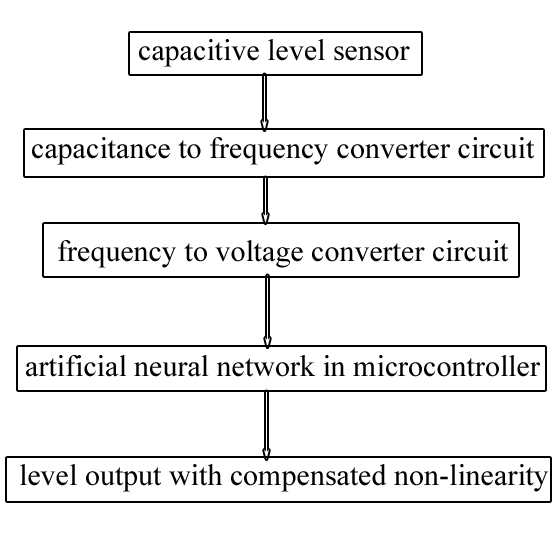
\includegraphics[width=8cm]{blockdiagram.png}
\centering
\caption{Block Diagram}\label{Fig4}
\end{figure}
\begin{figure}[h]
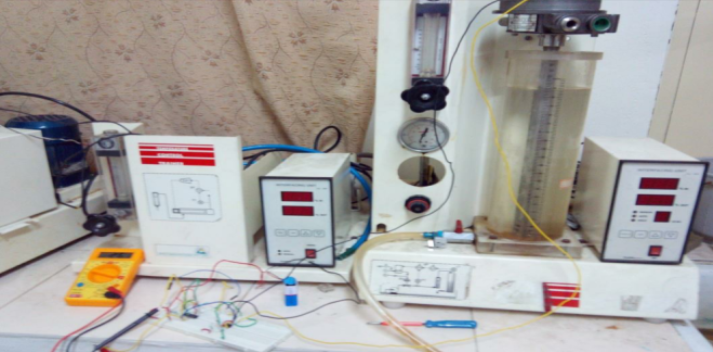
\includegraphics[width=8cm]{setup.png}
\centering
\caption{Experimental Setup}\label{Fig5}
\end{figure}

\section{Results}
\begin{table}
\begin{center}
  \begin{tabular}{ | c | c  | c | c |}
    \hline
    Method & Accuracy  & Function used & no of \\
    &&&neurons\\ \hline
    Back Propagation  & 99.8\% & tansig& 4 \\ 
    (Feed forward &&& \\
     Single layer ANN)&   &    &     \\ \hline
    ELM(Feed &98\% & sig &10\\ 
     forward Single &&& \\ 
     layer ANN)&&&\\ \hline
    RBF(Feed forward&99.84\%& gaussian& 13\\  
    Single layer ANN)&& &\\
    \hline
  \end{tabular}
\caption{Results\label{tab:b}}
\end{center}
\end{table}
Sensor output with water is 92.7\% linear, where as with soap solution it is 87\% linear. After training the single layer neural networks with methods shown in Table 2 with the ideal response of the capacitive sensor without any noise, the results which are obtained is shown in Table 2. 

%%PLOTS
\begin{figure}[h]
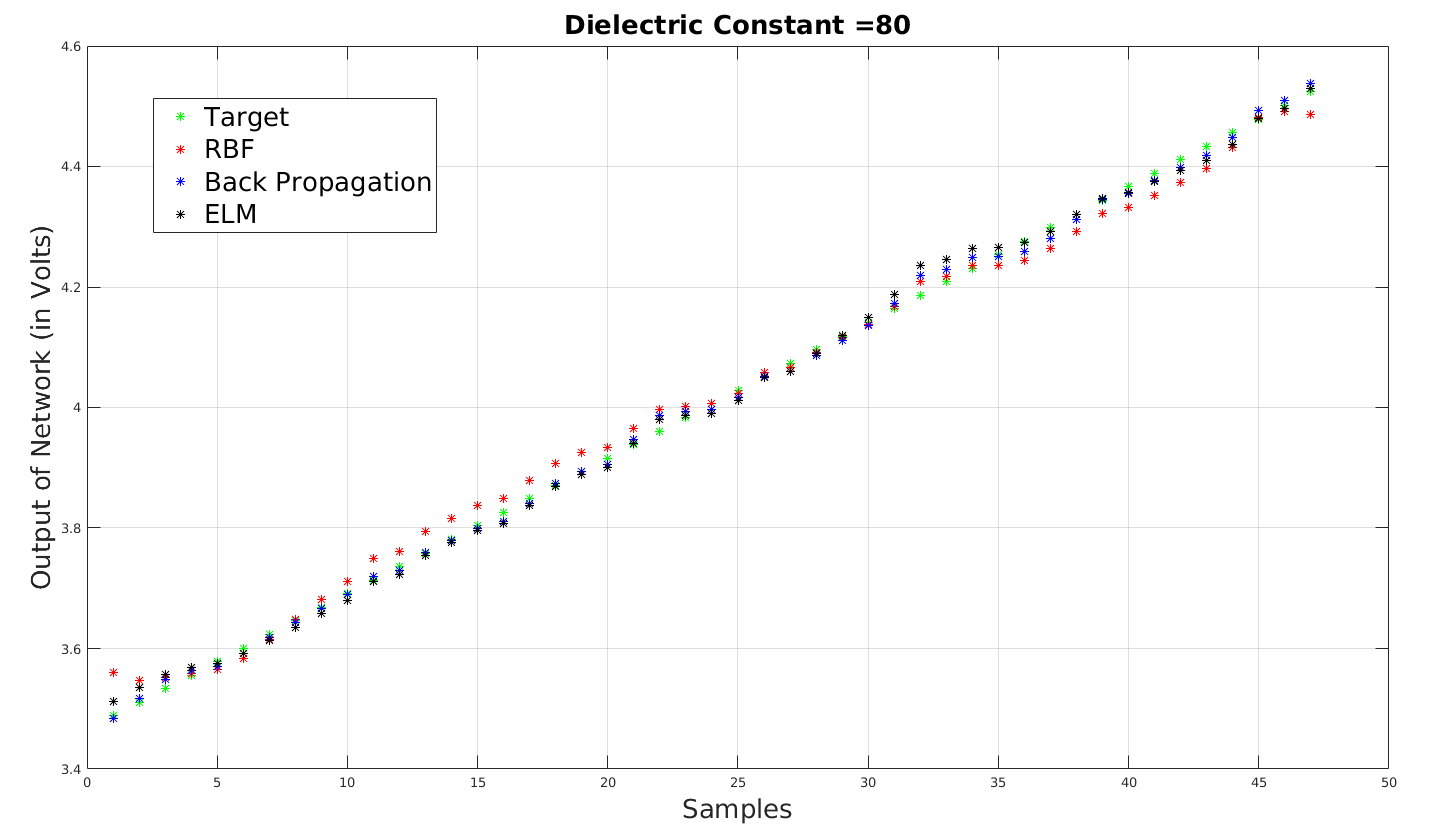
\includegraphics[width=8cm]{result1.png}
\centering
\caption{Response of network with dielectric constant 80}\label{Fig6}
\end{figure}

\begin{figure}[h]
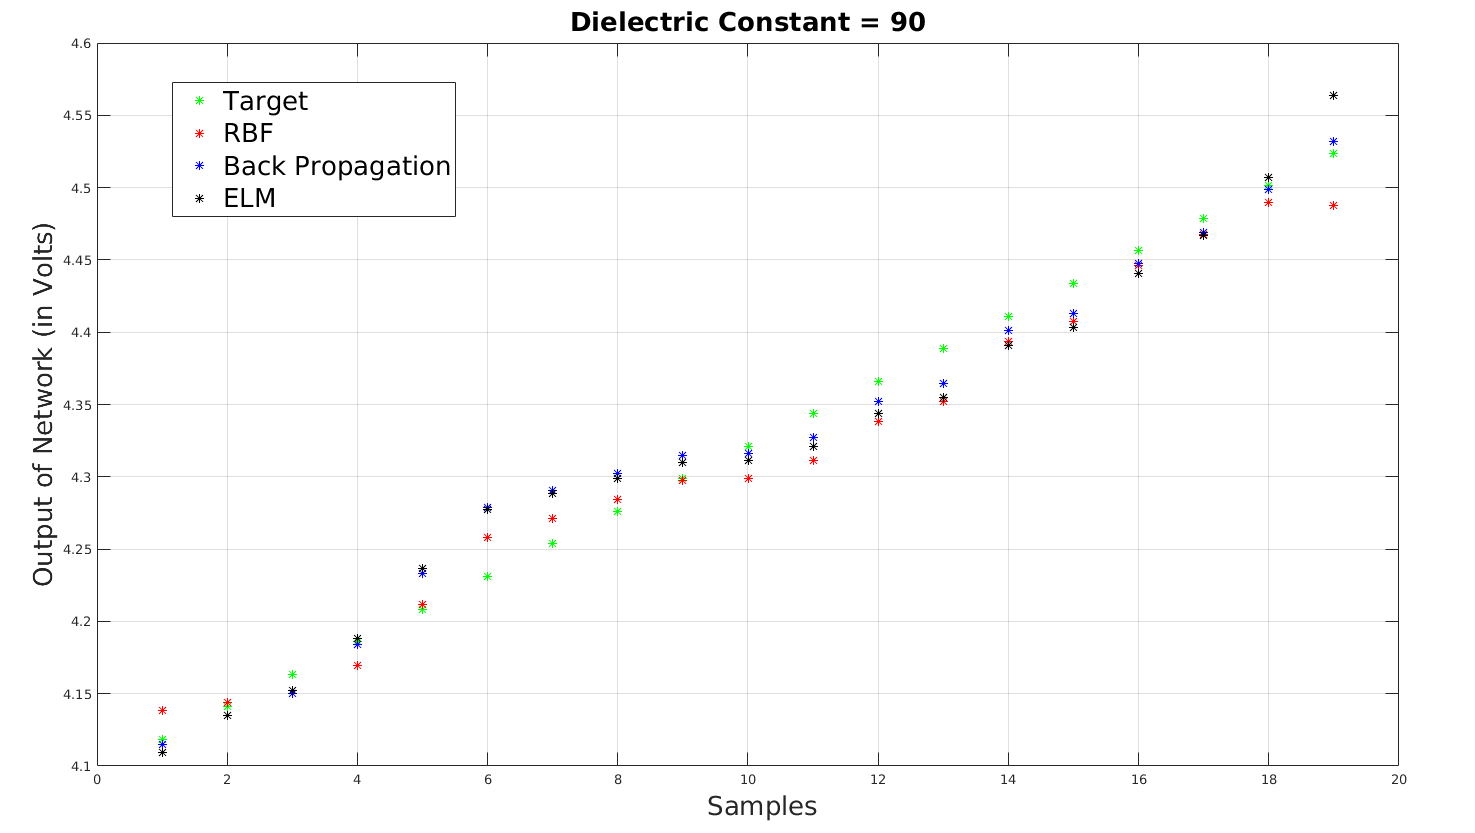
\includegraphics[width=8cm]{result2.png}
\centering
\caption{Response of network with dielectric constant 90}\label{Fig7}
\end{figure}
The response of the networks with two different liquids are shown in Figure 6 and Figure 7.


\section{Conclusion}
All the single layer feed forward neural network, were on the same idea of support vector regression where the 
inputs are mapped to higher dimensions using kernals which we choose in the hidden layer, where classification or regression can be done easily using linear interpreters. \\
Here the response of the capacitive sensor is almost linear but with very small deviations. Where this noise is best interpolated using the tansig kernal compared to others, with just four neurons.\\

\begin{thebibliography}{1}

\bibitem{}
Dempsey, G. L., et al. emph{Control sensor linearization using artificial neural networks.}\hskip 1em plus
  0.5em minus 0.4em\relax Analog Integrated Circuits and Signal Processing 13.3 (1997): 321-332.
\bibitem{}
Patra, Jagdish Chandra, Alex C. Kot, and Ganapati Panda. \emph{An intelligent pressure sensor using neural networks.} \hskip 1em plus
  0.5em minus 0.4em\relax Instrumentation and Measurement, IEEE Transactions on 49.4 (2000): 829-834.
\bibitem{}
Ji, Tao, Qingle Pang, and Xinyun Liu. \emph{An Intelligent Pressure Sensor Using Rough Set Neural Networks.}\hskip 1em plus
  0.5em minus 0.4em\relax Information Acquisition, 2006 IEEE International Conference on. IEEE, 2006. 
\bibitem{}
Medrano-Marqués, Nicolás J., and Bonifacio Martin-del-Brio. \emph{Sensor linearization with neural networks.}\hskip 1em plus
  0.5em minus 0.4em\relax Industrial Electronics, IEEE Transactions on 48.6 (2001): 1288-1290.
\bibitem{}
Khosravi, Mahdi, and Amir Abolfazl Suratgar. \emph{A model of optical micro electro mechanical pressure sensor using artificial neural networks.}\hskip 1em plus
  0.5em minus 0.4em\relax Electrical Engineering (ICEE), 2011 19th Iranian Conference on. IEEE, 2011.
% \bibitem{}
%  Khosravi, Mahdi, and Amir Abolfazl Suratgar. \emph{A model of optical micro electro mechanical pressure sensor using artificial neural networks.}\hskip 1em plus
%   0.5em minus 0.4em\relax Electrical Engineering (ICEE), 2011 19th Iranian Conference on. IEEE, 2011.

\end{thebibliography}




% that's all folks
\end{document}


